% !TEX encoding = UTF-8 Unicode
% !TEX root = ../thesis.tex
% !TEX spellcheck = en-US
%%=========================================



\chapter{Background}

\section{Glossary?}

\section{Augmented Reality}
(Jentoft, 2020) AR can be defined as a system that fulfills three basic features: a combination of real and virtual worlds, real-time interaction, and accurate 3D registration of virtual and real objects.

\subsection*{Disambiguation of some acronyms}\label{chap:armrxr}
As a new field, this field suffers from naming disagreements. This is a confusing reality which needs to be addressed. There are differing view of what each acronym refers to, and even what they stand for. I will overlook most of this discussion, and simply explain what is meant by each acronym in the scope of this project.

\paragraph*{AR}\label{para:ar} Augmented Reality, exercises which implement a see-through effect to display 3D visuals on top of the real-world. The idea of holograms is a good stand-in for the effect of AR. This is the term which will be most used in this project. 

\paragraph*{MR}\label{para:mr} Mixed Reality, anything within the spectrum between reality and pure visual 3D graphics, which blends computer generated visuals and reality. While the term was not invented by Microsoft\footnotemark, it is a term strongly associated with them, and in this project the term MR will generally only be used as a reference to Microsoft's products or concepts. There term is also used by some as a subset of \nameref{para:ar}, so in conclusion it is a somewhat controversial term. 

\footnotetext{In fact the term was coined by \citet{Milgram1994}, in this exact meaning.}
% That is at least what Microsoft is pushig for 

\paragraph*{XR}\label{para:xr} Extended Reality, much like \nameref{para:mr} this includes the whole spectrum of experiences blurring the line between the real and the virtual. However it does not have the Microsoft taint, nor the confusion of that term. And thus it is a more acceptable term, and it is what will be used here to describe the spectrum.

\paragraph*{VR}\label{para:vr} Virtual Reality, is enclosed experiences which completely surrounds the user within a computer generated world. This is a generally uncontroversial term and will be used for applications running on devices like the Oculus Rift and the HTC Vive.


\section{Graphics and Rendering}

\subsection*{Rasterization, Polygons and 3D models}

{
    \color{BrickRed}
    I feel that there is some misunderstanding about what a 3D model is.
    Maybe go in-depth about what I mean by 3D model. I have probably already used the term for different things.
}
% Three-dimensional graphics 
% The conversional rendering pipe-line

\section{Neuro stuff}

\subsection*{Ethics of dissection}\label{chap:ethics}

\subsection*{The Waxholm Space Atlas of the Sprague Dawley Rat Brain}\label{chap:ratbrain}

{
    \color{BrickRed}
https://www.nitrc.org/projects/whs-sd-atlas
\begin{itemize}
    \item What is a atlas
    \item WHS and ratbrain is open, used and developed by NTNU St Olavs and UiO 
    \item Waxholm Space Atlas of the Sprague Dawley Rat Brain 
    \item Discuss difference between graphical 3D model and 3D atlas
\end{itemize}
}


%  In this pursuit we will also make use of high-resolution 3D imagery of a rat brain (see \autoref{chap:ratbrain}).  

This project makes use of high-resolution 3D-models of a rat brain. This brain model has been captured and manually delineated\footnotemark[1] by a collaboration between research groups at the University of Oslo and NTNU, and is in fact a highly accurate volumetric representations of the rat brain. This model is an open access community resource, intended as a free tool for education and research\footnotemark[2]. Within the convectional rasterization rendering pipe-line of Nevrolens, a polygonal asset derived from this volumetric model is naturally used. 

\footnotetext[1]{Delineation refers to the process of clearly defining different structures in the brain into separate namable parts.}
\footnotetext[2]{https://www.nitrc.org/projects/whs-sd-atlas}

The model is simply referred to as \textit{The Waxholm Space Atlas of the Sprague Dawley Rat Brain}. What follows is a brief explanation of each confusing part of the this name. 

\subsubsection*{Waxholm Space}\label{chap:whs}
\begin{wrapfigure}{R}{0.40\textwidth} 
    \centering
    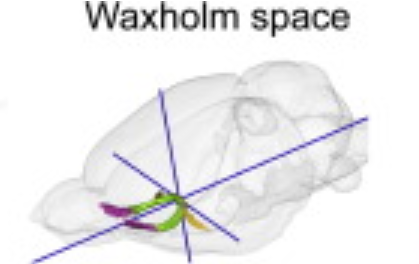
\includegraphics[width=0.30\textwidth]{fig/waxholmspace}
    \caption{\raggedright WHS \citep{WaxholmRatBrain2014}}
    \label{fig:waxholmspace}
\end{wrapfigure}

Waxholm Space (WHS) is a vector space defined as a standard reference space for the mouse brain and the rat brain \citep{WaxholmWithSimpleAbstract2013}. Its use as a coordinate system simplifies interoperability across atlases. It was developed by International Neuroinformatics Coordinating Facility (INCF) for the mouse brain, and has further been implemented in the rat brain by \citet{WaxholmRatBrain2014}. The following is the formal definition of WHS:


%  International Neuroinformatics Coordinating Facility (INCF) Digital Atlasing Project
\begin{quote}
\textit{
The coordinate system for WHS is defined as a continuous Cartesian system with the origin in the brain determined by 
\begin{itemize}
    \item the anterior commissure (AC) at the intersection between the mid sagittal plane,
    \item a coronal plane passing midway (rostro-caudal) through the anterior and posterior branches of AC, and
    \item a horizontal plane passing midway through the most dorsal and ventral aspect of the AC.
\end{itemize}
}
\citet{WaxholmSpaceAndMouseBrain2011}
\end{quote}

\noindent
\autoref{fig:waxholmspace} visualizes the axes through origin of WHS in the brain of a rat. Within the scope of this project WHS will be the local space of the rat brain model implemented in Nevrolens.

\subsubsection*{Brain Atlas}\label{chap:atlas}

A brain atlas is a composite representation based on one or more datasets of a given brain. An atlas generally has the function of highlighting some specified aspects and relations in the brain, and is a convectional tool in neuroscientific research \citep{Toga2000_AtlasBasics}. The convectional atlas is based on micrometer scale sliced sections in the brain, effectively creating two-dimensional layers through the brain. While functional, this "turns the brain into a book". Three-dimensional digital atlas are however relative newcomer on the neuro-imagery scene, by employing magnetic resonance imaging (MRI) and diffusion tensor imaging (DTI) the resulting atlases are complete volumetric representation of the subject brain \citep{WaxholmRatBrain2014}. 

This volumetric model is the basis for the delineated 3D-model used in Nevrolens.


\subsubsection*{Sprague Dawley}

Its a strain of laboratory rat.




\section{Equipment}

\subsection*{HoloLens 2}


\section{Tools}\label{chap:tools}


\subsection*{Unity}\label{chap:unity}

\begin{figure}
    \centering
    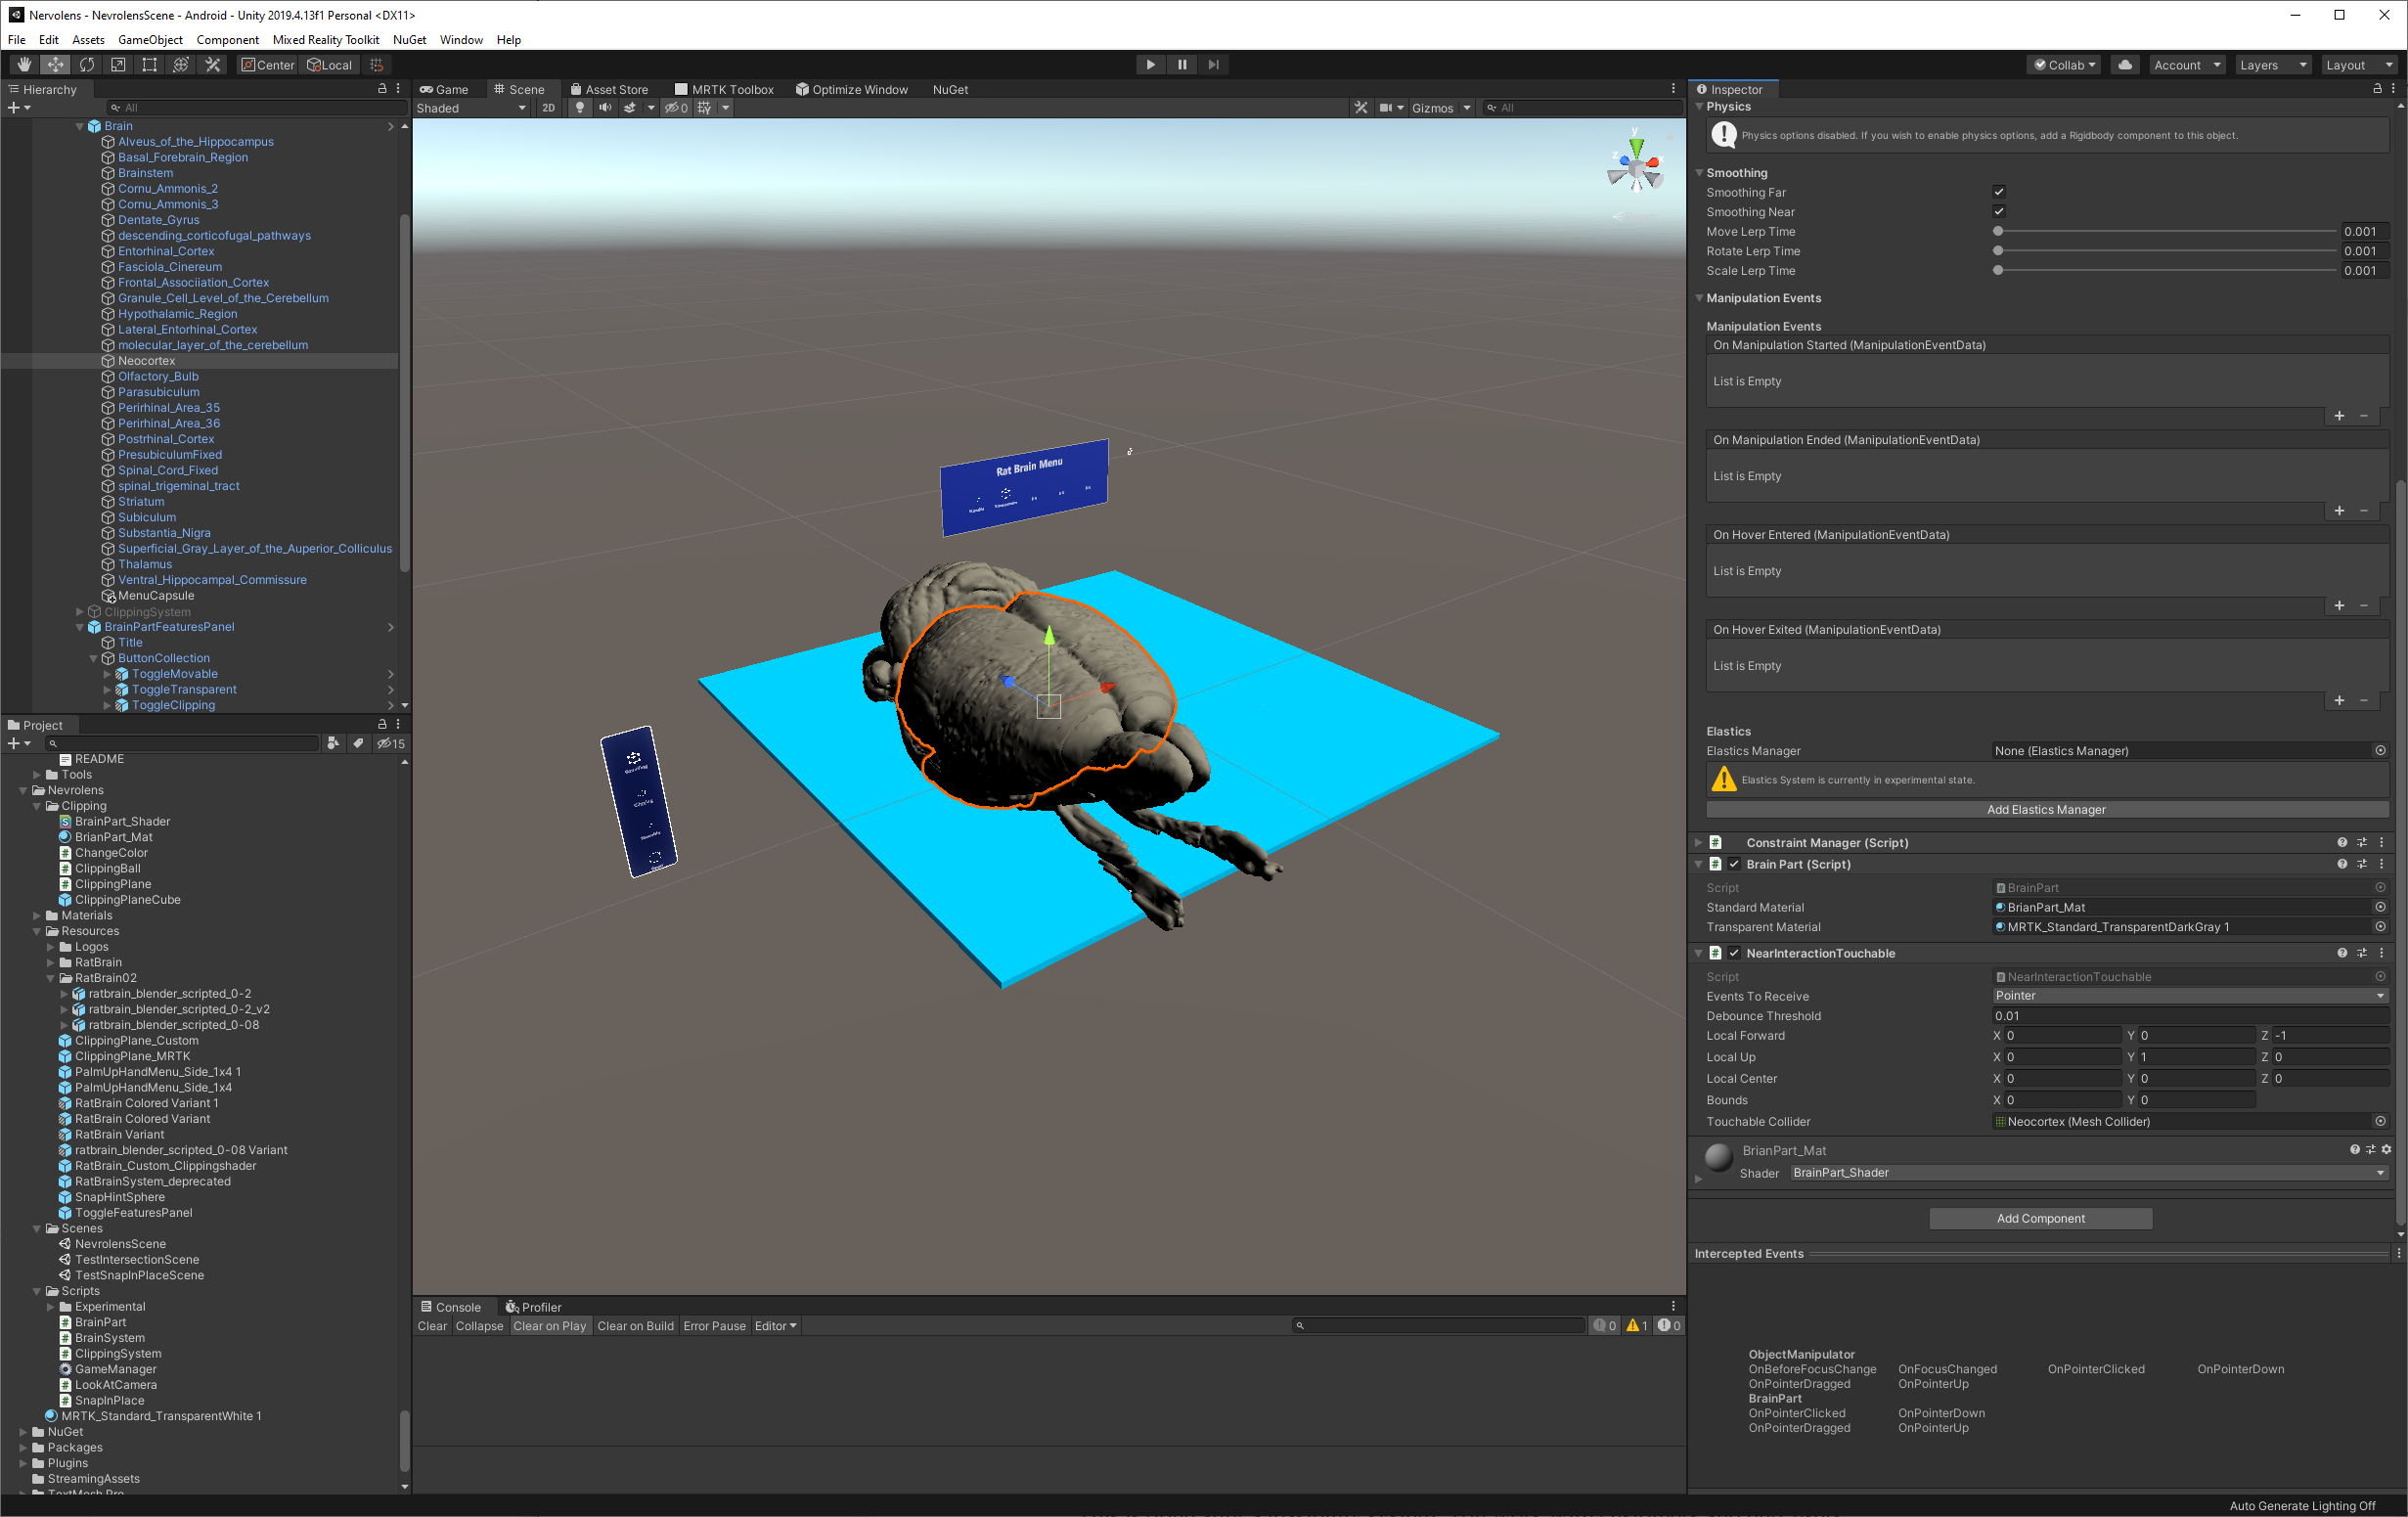
\includegraphics[width=\textwidth]{fig/unity_example.png}
    \caption{Unity 2019.4.13f1 running Nevrolens}
\end{figure}

Unity is a game engine for developing 2D and 3D games. It has grown to become the most popular game engine used by single developers and small development teams because of its ease of use and simple licensing terms for independent developers. Because of its popularity  and ease of use Unity has become a platform for 3D development within more widespread fields than video gaming, such as engineering, moviemaking and architecture. 
Within this project the critical reason for choosing Unity for our 3D development is the exceptional support for the HoloLens product line. As seen in the \autoref{chap:mrtk}, Microsoft has poured resources into developing a "relatively" robust open framework for using Unity to develop for HoloLens. 
Alternatives to using Unity are slim, but one could be to use Unreal Engine, an 3D game engine with great support for VR and AR in general, however the support for HoloLens specific tools like \nameref{chap:mrtk} is limited\footnote{Microsoft has a version of MRTK for Unreal, called \href{https://github.com/microsoft/MixedRealityToolkit-Unreal}{MRTK-Unreal}. It seems to be stale however, not having any updates in the last six months in the time of writing.}.
% An alternative to using Unity wo

\subsection*{Mixed Reality Toolkit}\label{chap:mrtk}
Mixed Reality Toolkit (MRTK) is a open source, Microsoft-driven framework for Mixed Reality (MR) development. In practice it is Microsoft's SDK for HoloLens development, greatly simplifying development related to interaction, user interface and  [\dots]. As it is a framework for MR in general, it supports other platforms like Android, iOS and VR devices such as HTC Vive and Oculus Rift with OpenVR. 
An alternative to using MRTK would be to us XRTK which is a community-driven fork of MRKT. Thought such a choice would be an exercise of free software principles, it also lends it self to better support for some devices, like the MagicLeap.



\subsection*{Blender}

Blender is a 3D modeling application, it is free open source software and is has a wide set of functionalities for 3D modeling, animation, rendering and optimization. Till now this project has only made use of one tool in Blender, \textit{decimation}, the process of simplifying the polygon count of a 3D model. This has been done by scripting, simply because Blender does not have a built-in way to apply a modifier on multiple objects\footnote{Or at least I didn't find any such solution.}. \autoref{item:blenderscript} showcases my use of Blender in its entirety.


\begin{lstlisting}[language=python, label={item:blenderscript}, caption={Blender script applying a decimate modifier to all relevant objects in a scene.}]
import bpy # importing the blender python library

def decimate(ratio, replace = True):
    # Finds all objects and filters irrelevant objects from the FBX 
    brainparts = [n for n in bpy.data.objects \
        if n.name not in ("Camera", "Light")]

    for part in brainparts:
        mod = 0
        # Finds all decimate modifiers on each brainpart
        decimate_mods = [n for n in part.modifiers \ 
           if n.type == 'DECIMATE']
        if decimate_mods and not replace:
            mod = decimate_mods[0]
        else:
            if replace: 
                # Removes all decimate modifiers from the brainpart
                for m in decimate_mods:
                    part.modifiers.remove(m)
            mod = part.modifiers.new(type='DECIMATE', name='Decimate')
            mod.decimate_type = 'COLLAPSE'
        # Sets the specifies strength to the decimate operation. 
        mod.ratio = ratio
# Calls function with given decimate strength.
decimate(0.08)
\end{lstlisting}

\subsection*{Photon}\label{chap:photon}
Photon is the state of the art networking library for Unity. It can manage everything from voice chat to interaction over network. This has not jet been used in the project, but will be referred to in \nameref{chap:futurework}. 

\subsection*{Git}
Git flow, Gitmoji, GitKraken, Git gud 

\subsection*{GitKraken Boards}
Kanban and such \\
Used both / separately for Nevrolens and Project thesis.




\section{Related work}

\subsection*{VRVisualizer}\label{chap:vrvis}
% VRVisualizer is the name of the research product of the master thesis \citet{Elden2017}.

\subsection*{HoloAnatomy}

\subsection*{Insight Heart}

\subsection*{SphenoBlock?}

\subsection*{Noe HoloCare stuff?}

